



\section{Application design}
The penetration testing tool is chosen to be a desktop based GUI application. Desktop applications will have no dependencies on browsers. Server side - client side code complications and JavaScript engine dependencies are also removed. It is planned that all libraries and resources required for the application to run would be included in the final deliverable, thus increasing portability and reducing setup complexity. Additional features as automatic update service and application error scan is planned in order to keep software up to date by using git repository as a code base.

Application will implement modular design to re-use existing penetration tools and follow usage-centered design principles. In order to add a tool to the tool set, a user will have to define an interface/wrapper for the new tool. The wrapper will contain instructions on how to convert GUI input to tool specific commands as well as interpret tools output. This design allows flexibility and makes no assumptions about individual tool input or output. By prioritizing usability and clarity the application will remain user friendly and minimize new users learning curve \cite{user}.

It has been decided that the application will be written in Python. Python is a dynamic scripting language suitable for rapid development and prototyping. There will be no learning curve to use it as work experience is already present. Graphic User Interface will be developed using PyQT library as it is highly customize and popular between Python developers. Python is also by default present in the majority of Linux distributions, therefore no additional setup will be required. Other alternatives as Java, JavaScript and C++ were considered but were dismissed due slower development cycle, steeper learning curve or lack. One may point out Python lesser performance as a disadvantage but as the majority of computationally heavy tasks will be executed by other tools that does not make any difference.

A UML diagram present describes general application structure.

\begin{figure}[h!]
\caption{UML diagram}
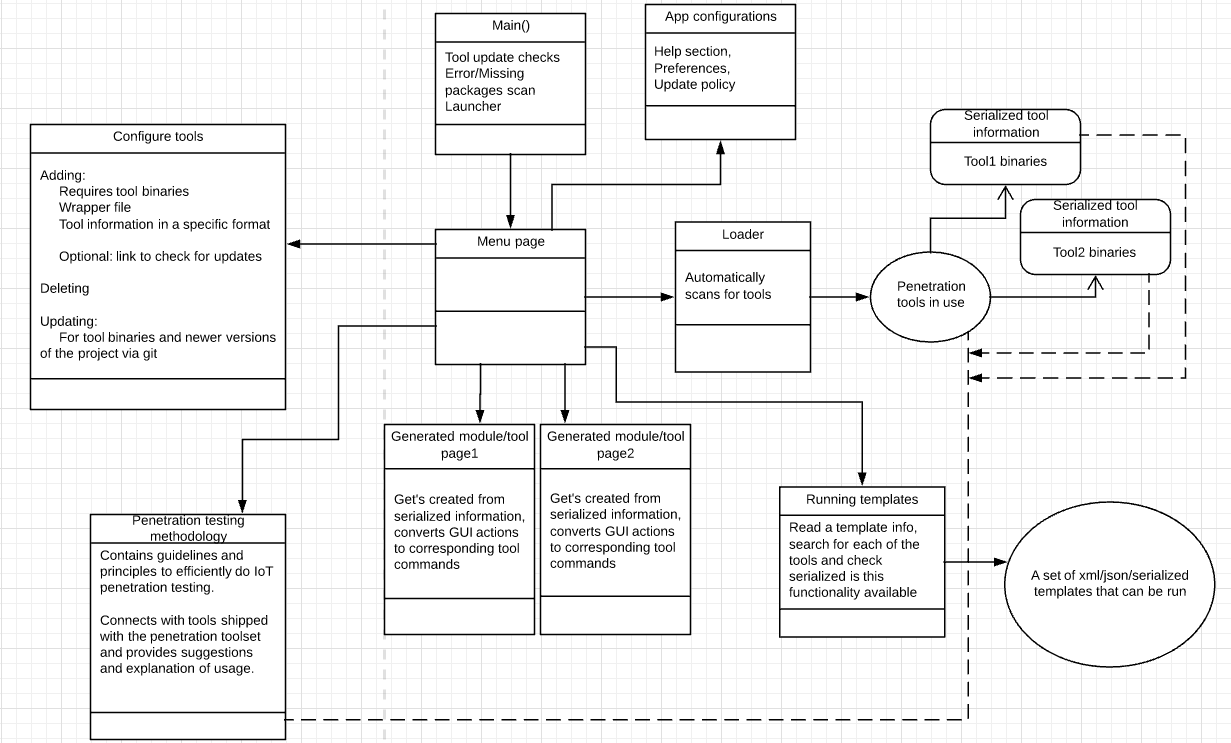
\includegraphics[width=\linewidth]{UML-diagram}
\centering
\end{figure}

\section{Remaining work}

Work completed up to this point and the remaining work is visualized using Gannt chart. The application design and background research phases are completed. The remaining development time will be mostly divided into sprints of 10-14 days in order to assign time for inevitable other module assignments. Each sprint will have a predefined set of tasks prioritized in Agile manner. After the sprint is completed planned functionality is supposed to be fully functional and tested to constantly add value. The Christmas period, January exam period and Easter periods are planned in looser manner in order to accommodate vacations, assess progress and re-think design decisions. The last weeks of the project are reserved for writing final report.

\begin{figure}
\caption{Gannt chart}
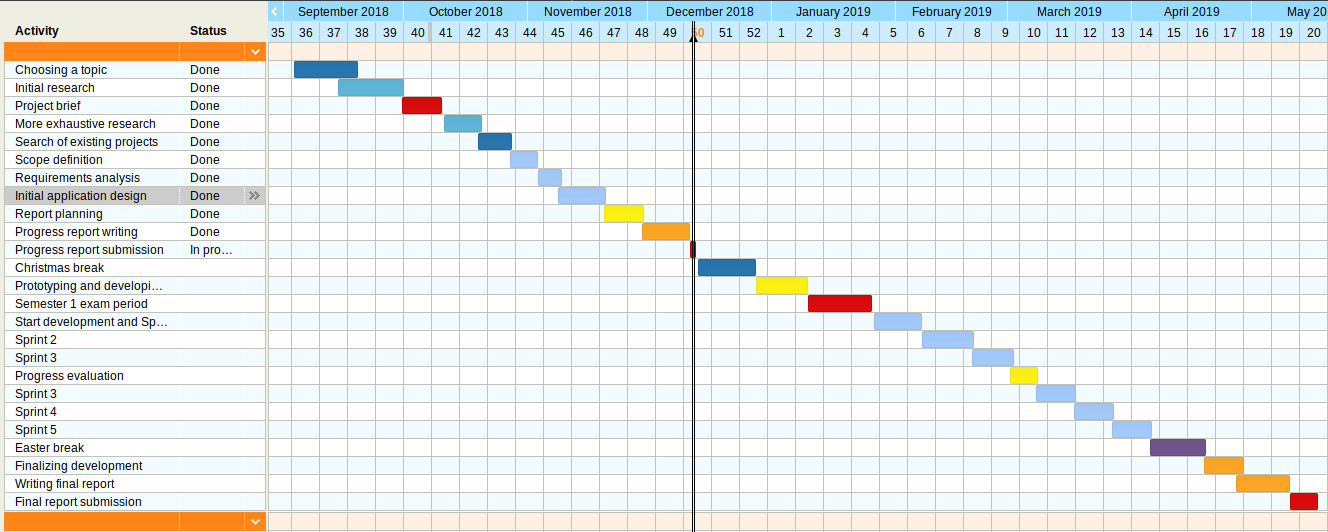
\includegraphics[width=\linewidth]{Gannt}
\centering
\end{figure}


\subsection{Risk analysis}
Probability and Impact are rated in a scale from 1 to 5.

\def\riska{Loss of source code at some stage of development}
\def \probabilitya {1}
\def \impacta {4}
\def \mitigationa {Use of remote source control  repository to frequently record every stage of the development, thus being able to recover it if needed. }

\def\riskaa{Unable to fulfill all of the requirements due to technical implemention difficulties}
\def \probabilityaa {3}
\def \impactaa {2}
\def \mitigationaa {During the start of development process requirements will be split into tasks, divided into sprints and ranked using Agile methodology, therefore ensuring that core functionality will be implemented first and a working proof of concept is available at the end of the project }

\def\riskaaa{Loss of development time due to other course modules}
\def \probabilityaaa {2}
\def \impactaaa {2}
\def \mitigationaaa {Dedicate fixed amount of time every week for the project in order to keep up with the schedule }

\def\riskaaaa{Some part of the project taking up significantly longer that expected}
\def \probabilityaaaa {3}
\def \impactaaaa {2}
\def \mitigationaaaa {Re-evaluate task importance and readjust development schedule in order to deliver functional prototype }

\def\riskaaaaa{Unable to complete adequate application testing due to technical or time limitations}
\def \probabilityaaaaa {3}
\def \impactaaaaa {3}
\def \mitigationaaaaa {Complete limited or partial testing concentrating on core functionality, document causes and reasoning. If difficulties arise in early stages of development  due to technical limitations, seek support from university staff that have more experience in similar situations. }

\begin{table}
	\centering
	\begin{tabular}{ |m{5cm}|m{2cm}|m{1cm}|m{6cm}| } 
		\hline
		Risk & Probably & Impact & Mitigation \\ 
		\hline
		\riska & \probabilitya & \impacta & \mitigationa \\ 
		\hline
		\riskaa & \probabilityaa & \impactaa & \mitigationaa \\ 
		\hline
		\riskaaa & \probabilityaaa & \impactaaa & \mitigationaaa \\ 
		\hline
		\riskaaaa & \probabilityaaaa & \impactaaaa & \mitigationaaaa \\ 
		\hline
		\riskaaaaa & \probabilityaaaaa & \impactaaaaa & \mitigationaaaaa \\ 
		\hline
	\end{tabular}
	\caption{\label{tab:risk_ana} Risk analysis}
\end{table}